\documentclass[conference]{IEEEtran}
\IEEEoverridecommandlockouts
% The preceding line is only needed to identify funding in the first footnote. If that is unneeded, please comment it out.
\usepackage{cite}
\usepackage{amsmath,amssymb,amsfonts}
\usepackage{algorithmic}
\usepackage{graphicx}
\usepackage{textcomp}
\usepackage{xcolor}
\graphicspath{{./Screenshots}}

\def\BibTeX{{\rm B\kern-.05em{\sc i\kern-.025em b}\kern-.08em
T\kern-.1667em\lower.7ex\hbox{E}\kern-.125emX}}
\begin{document}

    \title{Dynamic Routing using P4 Switches and the FABRIC Measurement Framework\\}

    \author{\IEEEauthorblockN{Shikhar Gupta}
    \IEEEauthorblockA{School of Computing \& Augmented Intelligence \\
    Arizona State University \\
    sgupt330@asu.edu}
    \and
    \IEEEauthorblockN{Kiran Sthanusubramonian}
    \IEEEauthorblockA{School of Computing \& Augmented Intelligence \\
    Arizona State University \\
    ksthanus@asu.edu}
    }
    \maketitle

    \begin{abstract}
        The ecosystem of application functionality built around programmable
        switch hardware is growing at a rapid pace in recent times, fueled by
        the advent of reconfigurable match-action table technology.
        This new class of devices is capable of simultaneously delivering
        basic computation and line-rate forwarding at a reasonable cost.
        Network monitoring systems include software and hardware tools that can track various aspects of a network and its operation, such as traffic, bandwidth utilization, and uptime. These systems can detect devices and other elements that comprise or touch the network, as well as provide status updates. We present an approach where with the help of the metric gathered we switch the routes between the hosts in real time without requiring the assistance of the network operator.

    \end{abstract}

    \begin{IEEEkeywords}
    \end{IEEEkeywords}


    \section{Introduction}
    Rapid progress has been made in programmable data planes in the past few years. The P4 programming language \cite{b1} has been a pivotal driving factor in making the programmability of switches protocol and hardware independent. P4 enhances the use of Software Defined Networking and the OpenFlow API to configure forwarding devices and network behavior determination in a "top-down" approach. P4 has been used in areas such as DDoS attack prevention, improving network resilience paradigms \cite{b2}, load balancing, and traffic engineering. P4 switches have also been used as a backbone to create software systems for performance-based ISP routing.

    This project will create a dynamic routing experiment using BmV2 P4 Switches on the FABRIC Testbed. The FABRIC Testbed is a programmable research infrastructure that can be used for large-scale research. The resources of the infrastructure are used in the form of a slice.

    Network Monitoring technique is an important aspect of modern computer networks. These techniques give visibility into the network, enable better resource usage, and provide the ability to identify potential security threats on time. Active and passive network monitoring techniques have been used significantly to monitor networks. As a deep dive into network monitoring, the project will demonstrate the use of the FABRIC Measurement Framework Library (MFLib) \cite{b3}, to collect critical slice information by automatically adding monitoring software and services to the slice infrastructure.
    Mininet is also a great way to develop, share, and experiment with Software-Defined Networking (SDN) systems using OpenFlow and P4. It's a network emulator which creates a network of virtual hosts, switches, controllers, and links. Mininet hosts run standard Linux network software.
    Scapy is a Python program that enables the user to send, sniff and dissect and forge network packets. This capability allows construction of tools that can probe, scan or attack networks.
    In other words, scapy is a powerful interactive packet manipulation program. It is able to forge or decode packets of a wide number of protocols, send them on the wire, capture them, match requests and replies, and much more.



    \section{Problem Statement}
    This project will set up a routing experiment with a programmable switch Topology dynamically configured using P4. Using P4 we will modify routing tables on the switches in real time, which will form the basis for examining the packet flow between two hosts connected via multiple routing paths. The entire topology will be first deployed using virtual machines, virtual network interfaces(Mininet) and scapy will be used to generate traffic. Our initial work with mininet and scapy will help build our algorithm to dynamically shift routes between hosts and will be further used for our experiment  where our infrastructure will be deployed as a slice on the FABRIC testbed infrastructure, and slice-level metrics will be collected, curated, and presented using the FABRIC measurements framework library which will be used for our algorithm.\\


    \section{Methodology}

    \subsection{Initial Setup}
    We start with the initial topology used for our experiments in Figure 1. 3 hosts in different subnets are connected to one switch. The switch is a programmable BmV2 P4 switch. Once we configure the routing tables on the P4 switch we can achieve L3 forwarding to forward traffic to the host on a different subnet. This initial setup will help us build the foundation of our project.

    \begin{figure}[h!]
        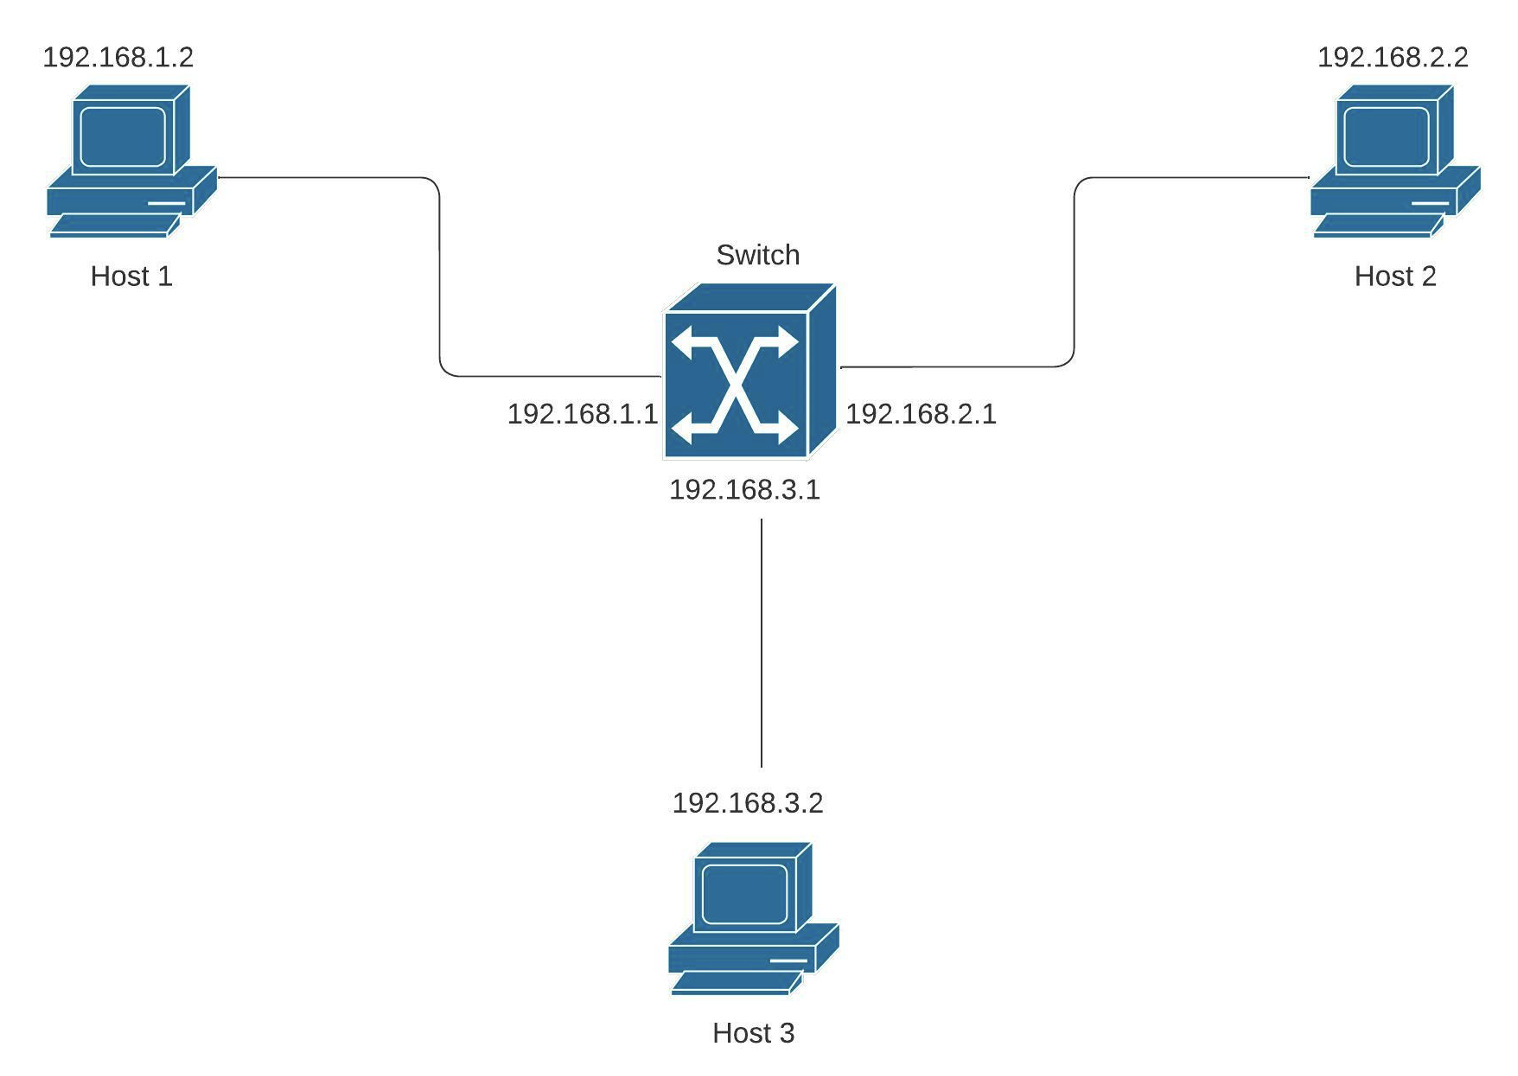
\includegraphics[scale=0.2]{Initial Switch topology.png}
        \centering
        \caption{Experiment Slice Topology}
    \end{figure}

    \subsection{Trraffic Generation}
    We will be using scapy as our traffic generator, to increase the load on the different routes between our hosts. Figure 2. shows the real-time graph of the metric(TCP packets) captured using prometheus and grafana, as we generate traffic using scapy.

    \begin{figure}[h!]
        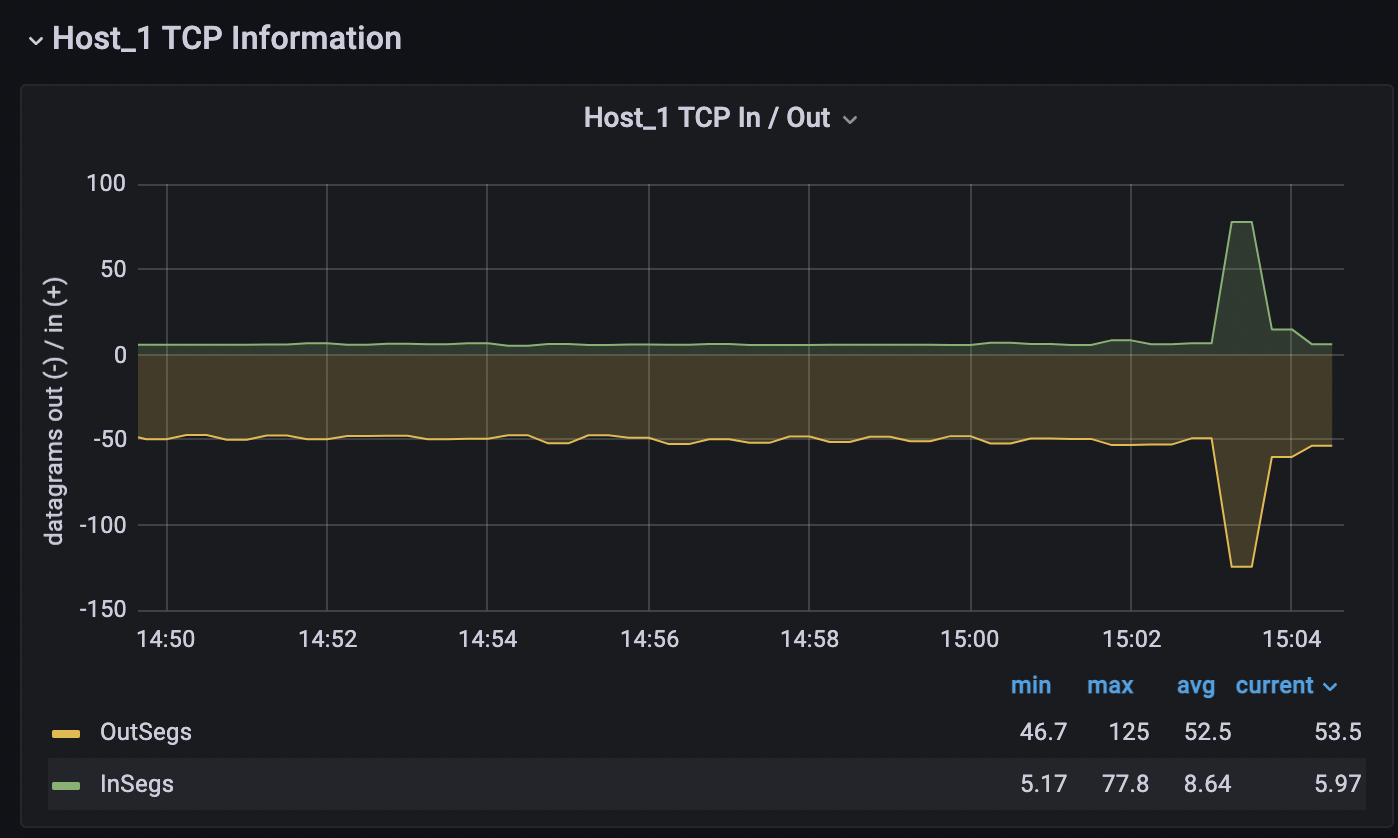
\includegraphics[scale=0.3]{Graph1.png}
        \centering
        \caption{TCP Packets in/out}
    \end{figure}

    \subsection{Metrics Collection using MFLib}
    The complete slice-level metrics will be measured using the MFLib API present in the FABRIC Testbed. The MFLib API enables us to have a definitive way to store our metrics using Prometheus, the logs using ElasticSearch (ELK stack), and visualize the collected data using Kibana and Grafana. The network monitoring node(meas\_node) in our infrastructure will collect and store the slice-level metrics like TCP/ICMP/UDP packets (in/out), queue length, system load, and network traffic load.

    \begin{figure}[h!]
        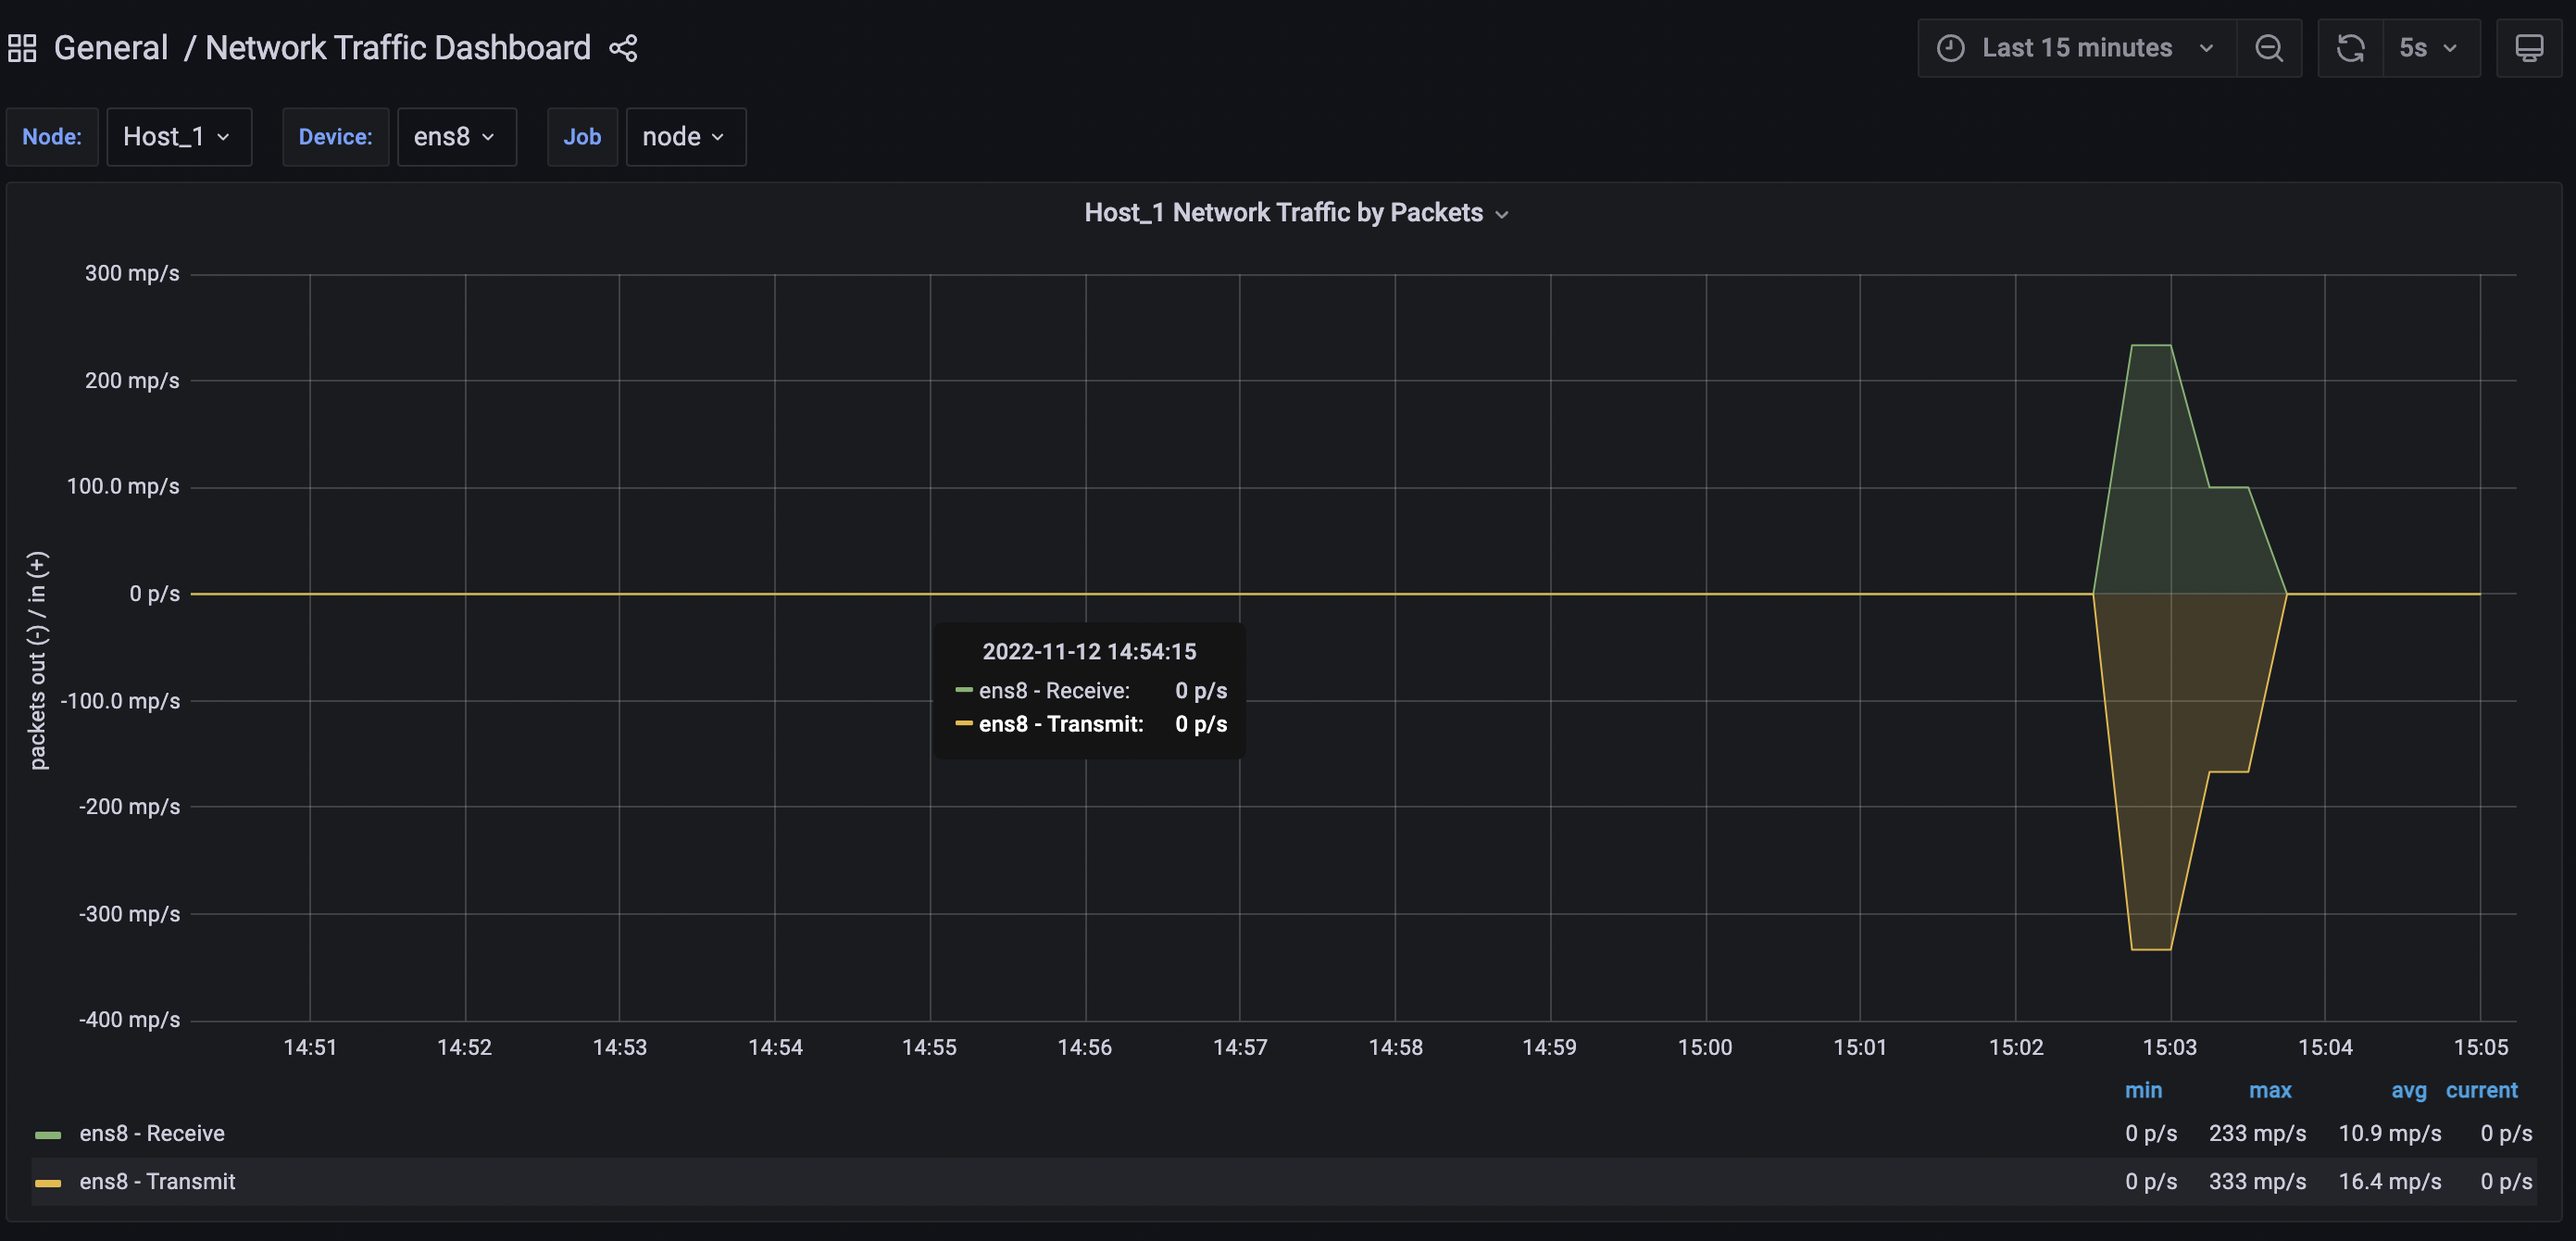
\includegraphics[scale=0.15]{Graph2.png}
        \centering
        \caption{Network Traffic on Host 1}
    \end{figure}

    \subsection{Final Experiment Setup}
    We describe the topology used for our experiments in Figure 2. The measuring node of our infrastructure provided by MFLib will act as the controller which will collect and store the metrics that will be used by our algorithm to configure the routing tables on the switches of our topology. As the switches defined are completely programmable BmV2 P4 switches, the routing tables on the programmable switch will be configured dynamically in such a way that it can alternate between the two available paths between the hosts. This will be achieved using CLI commands that our P4 code provides.
    The scope of this project is to have only 2 routes between the hosts, in a real-world scenario, there can exist more than 2 routes.

    \begin{figure}[h!]
        \centering
        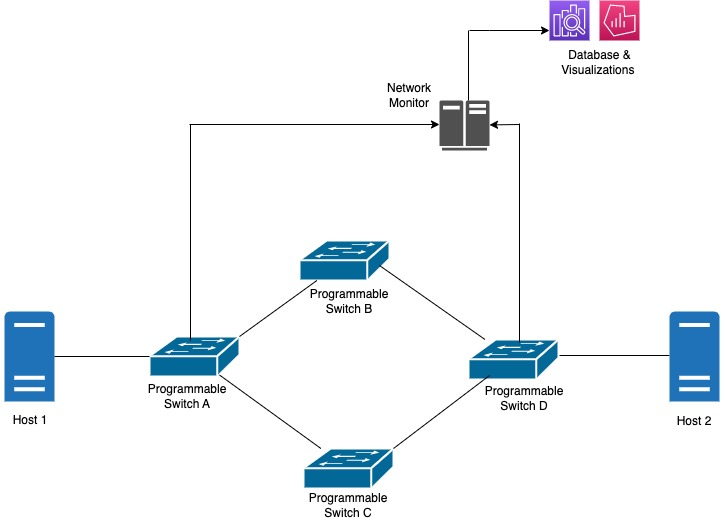
\includegraphics[scale=0.3]{Project_Proposal_Topology.jpeg}
        \caption{Experiment Slice Topology}
    \end{figure}


    \section{Project Deliverables}

    \subsection{Primary Objectives}
    \begin{enumerate}
        \item Walkthrough of P4 tutorials; implementing and deploying a basic P4 program on Mininet.
        \item Setting up the proposed topology on FABRIC.
        \item Implementing and deploying a basic P4 program on FABRIC.
        \item Implementing the entire telemetry system with minimal network and processing overheads and visualizing the telemetry gathered when the hosts communicate. This stage will also include writing a codebase using the MFLib API to continuously monitor and log slice information.
        \item Update routing tables present in the P4 switches in real-time based on the metrics we get from MFLib.
        \item Visualize the telemetry and slice information based on overall throughput and latency. We will also attempt to visualize a simulation showcasing the dynamic route-switching capability.
    \end{enumerate}

    \subsection{Stretch Objectives}
    \begin{enumerate}
        \item Implement the INT-based Telemetry System to monitor the entire slice topology.
        \item Collect and visualize the metrics and logs gathered using the INT Packets, P4 Switches, and the Network Monitor.
        \item Provide comparisons of the metrics gathered between the FABRIC Measurement Framework and the INT Framework.
    \end{enumerate}


    \section{Learning Outcomes}
    Our primary goal from this project is to gain a deep understanding of P4, its implementation details, and how to deploy P4 programs for data plane programmability. Our interest in P4 and the INT Framework stems from an appreciation for Dynamic Routing protocols and real-time Load Balancing systems. This project, if successful, could give us more insights into these core Networking topics.


    \section{Initial Results}
    Our preliminary goal is to toggle the routes between hosts dynamically and try sending ICMP packets between subnets. Once the P4 program is complied we can achieve our goal by adding/removing the routes in the table in the switch. Figure 6. shows the network packets forwarded before and after toggeling the route between the hosts.


    \begin{thebibliography}{00}
        \bibitem{b1} Pat Bosshart, Dan Daly, Glen Gibb, Martin Izzard, Nick McKeown, Jennifer Rexford, Cole Schlesinger, Dan Talayco, Amin Vahdat, George Varghese, and David Walker. 2014. “P4: programming protocol-independent packet processors”. SIGCOMM Comput. Commun. Rev. 44, 3 (July 2014), 87–95

        \bibitem{b2} Weverton Luis da Costa Cordeiro, Jonatas Adilson Marques, Luciano Paschoal Gaspary, “Data Plane Programmability Beyond OpenFlow: Opportunities and Challenges for Network and Service Operations and Management.” Journal of Network and Systems Management (September 2017).

        \bibitem{b3} Ilya Baldin, Anita Nikolich, Paul Ruth, Jim Griffioen, Kuang-Ching Wang, Inder Monga, and Tom Lehman, “FABRIC Measurement Framework Design,” v0.2

        \bibitem{b4} The P4.org Applications Working Group. Contributions from Alibaba, Arista, CableLabs, Cisco Systems, Dell, Intel, Marvell, Netronome, VMware, “In-band Network Telemetry (INT) Dataplane Specification,” Version 2.1, 2020-11-11

        \bibitem{b5} N. Van Tu, J. Hyun, and J. W.-K. Hong, "Towards ONOS-based SDN monitoring using in-band network telemetry," in Proc. 19th Asia–Pacific Netw. Oper. Manage. Symp. (APNOMS), Seoul, South Korea, Sep. 2017, pp. 76–81

        \bibitem{b6} N. V. Tu, J. Hyun, G. Y. Kim, J. -H. Yoo and J. W. -K. Hong, "INTCollector: A High-performance Collector for In-band Network Telemetry," 2018 14th International Conference on Network and Service Management (CNSM), 2018, pp. 10-18.
    \end{thebibliography}

\end{document}